\documentclass[15pt]{beamer}

\mode<presentation>
{
  %\usetheme{Singapore}
  %\usetheme{Malmoe}
  \usetheme{Pittsburgh}
  \usecolortheme{X}
  \setbeamercovered{transparent}
  \usefonttheme{serif}
}

\usepackage[utf8]{inputenc}
\usepackage{ucs}
\usepackage{xcolor}
\usepackage{graphics}
\usepackage{amsmath}
\usepackage[T1]{fontenc}
\usepackage{arev}
\usepackage{setspace}

\renewcommand{\arraystretch}{1.5}

\title
{Short Intro to AI}

\author{Adrienn Szabo}

\date
{\scriptsize{March 31. 2017}}

\begin{document}


\begin{frame}
    \titlepage
\end{frame}


\begin{frame}{TOC}
    \normalsize
    \tableofcontents
    % You might wish to add the option [pausesections]
\end{frame}


\section{What?}


\begin{frame}{What is Artificial Intelligence?}
    A huge research topic, always changing\dots
    \vspace{2mm}

    The \alert{AI effect}:

    \small
    \vspace{2mm}
    \begin{itemize}\itemsep0.8em
        \item ,,As soon as AI successfully solves a problem, the problem is no longer a part of AI.''
        \item ,,AI is whatever hasn't been done yet.''
        \item ,,Every time we figure out a piece of it, it stops being magical; we say, \emph{Oh, that's just a computation.} ''
    \end{itemize}
    \normalsize
\end{frame}


\begin{frame}{What is Artificial Intelligence?}
    \begin{itemize}\itemsep0.6em
        \item Self-driving cars
        \item Chatbots
        \item Modeling systems (weather forecast)
        \item Recommender systems
        \item Image recognition
        \item Speech recognition
        \item Human Language Translation
        \item etc.
        \item \alert{But no "General AI" (yet)}
    \end{itemize}
\end{frame}


\subsection{Supervised Learning}


\begin{frame}{Supervised Learning}
    A specific sub-area, where we build up a \alert{model}
    by showing it \alert{examples} with \alert{labels}.

    \vspace{3mm}
    \begin{itemize}\itemsep0.6em
        \item Artificial Neural Networks
        \item Bayesian Statistics
        \item Decision Trees, Random Forests
        \item Support Vector Machines
        \item etc.
    \end{itemize}
\end{frame}


\begin{frame}{Supervised Learning}
    \begin{center}
        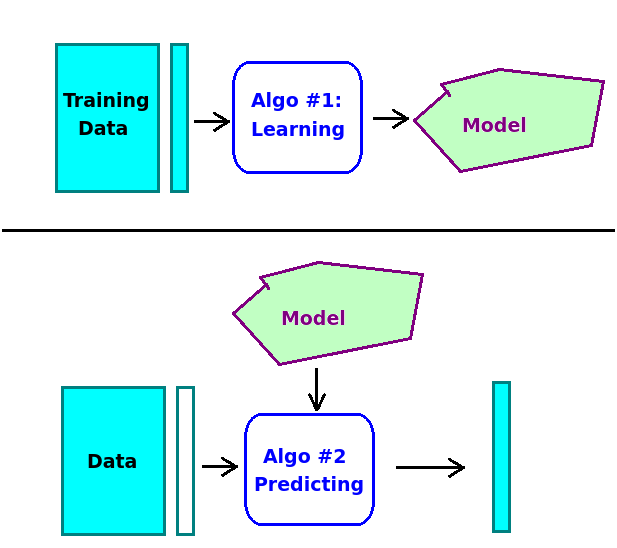
\includegraphics[scale=.5]{img/howitworks.png}
    \end{center}
\end{frame}

\begin{frame}{Two Types of Supervised Learning}
    \begin{center}
        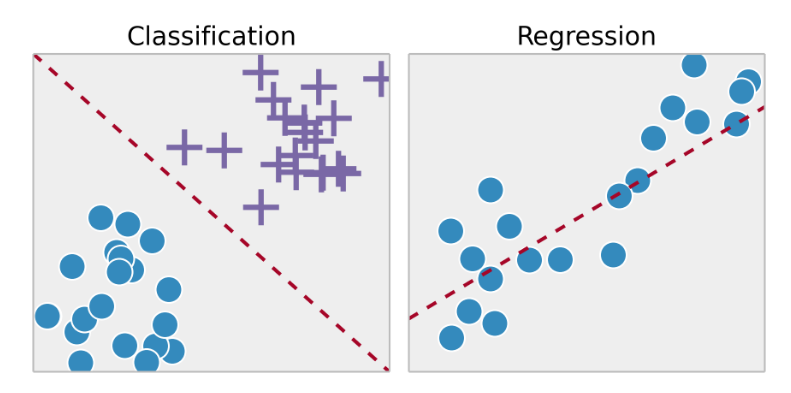
\includegraphics[scale=.5]{img/class_regr.png}
    \end{center}
\end{frame}


\section{How?}
\subsection{Example: Naive Bayes Classifier}


\begin{frame}{Example Task}
    \begin{columns}[c]
    \column{.57\textwidth}
        \hspace{8mm}\large{Binary classification:}
        \vspace{3mm}

        \normalsize
        \hspace{3.5mm}The task is to predict from \\
        \hspace{3.5mm}some binary \alert{features} if an \\
        \hspace{3.5mm}animal is a \alert{cow} or \alert{not a cow}.

        \vspace{1mm}

    \column{.43\textwidth}
        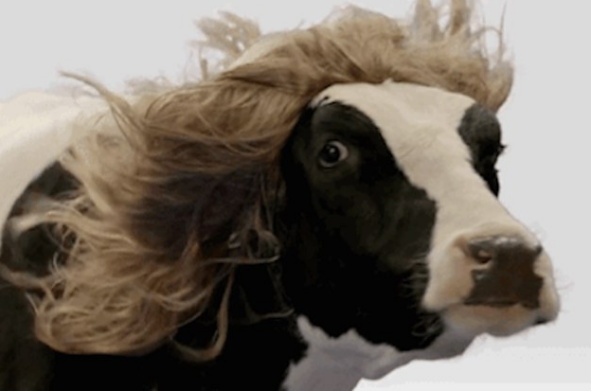
\includegraphics[scale=.28]{img/haircow.png}
    \end{columns}

    \vspace{4mm}

    The matrix we'll have (\alert{training dataset}):
    \vspace{2mm}
    \begin{itemize}\itemsep0.5em
        \item 7 binary descriptors or features (columns)
        \item 20 animals (rows)
        \item one row for each animal: features + label (1/0)
    \end{itemize}
\end{frame}


\begin{frame}{Example Task}
    The features (columns) of the data set:
    \vspace{2mm}
    \begin{itemize}\itemsep0.5em
        \item (0) Does it have four legs?
        \item (1) Does it have fur?
        \item (2) Is its color black and white?
        \item (3) Is its color black only?
        \item (4) Is its color white only?
        \item (5) Is its color 'other'?
        \item (6) Is it small (under 200kg)?
        \item (+) The label: is it a cow?
    \end{itemize}
\end{frame}


\begin{frame}{Example data row 1}
    \begin{columns}[b]
    \column{.61\textwidth} % column designated by a command
        \small
        \begin{itemize}\itemsep0.25em
            \item (0) Does it have four legs?
            \item (1) Does it have fur?
            \item (2) Is its color black and white?
            \item (3) Is its color black only?
            \item (4) Is its color white only?
            \item (5) Is its color 'other'?
            \item (6) Is it small (under 200kg)?
        \end{itemize}
    \column{.38\textwidth}
        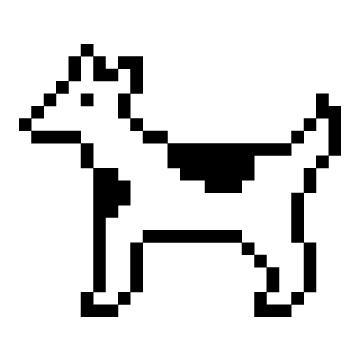
\includegraphics[height=30mm]{img/dog_01.jpg}
    \end{columns}

    \vspace{6mm}
    \normalsize
    \hspace{68mm}\texttt{[1,1,1,0,0,0,1]}
\end{frame}


\begin{frame}{Example data row 2}
    \begin{columns}[b]
    \column{.61\textwidth} % column designated by a command
        \small
        \begin{itemize}\itemsep0.25em
            \item (0) Does it have four legs?
            \item (1) Does it have fur?
            \item (2) Is its color black and white?
            \item (3) Is its color black only?
            \item (4) Is its color white only?
            \item (5) Is its color 'other'?
            \item (6) Is it small (under 200kg)?
        \end{itemize}
    \column{.38\textwidth}
        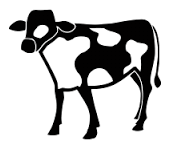
\includegraphics[height=30mm]{img/cow_2.png}
    \end{columns}

    \vspace{6mm}
    \normalsize
    \hspace{68mm}\texttt{[1,1,1,0,0,0,0]}
\end{frame}


\begin{frame}{Example data row 3}
    \begin{columns}[b]
    \column{.61\textwidth} % column designated by a command
        \small
        \begin{itemize}\itemsep0.25em
            \item (0) Does it have four legs?
            \item (1) Does it have fur?
            \item (2) Is its color black and white?
            \item (3) Is its color black only?
            \item (4) Is its color white only?
            \item (5) Is its color 'other'?
            \item (6) Is it small(under 200kg)?
        \end{itemize}
    \column{.38\textwidth}
        
\includegraphics[height=30mm]{img/worm_1.png}
    \end{columns}

    \vspace{6mm}
    \normalsize
    \hspace{68mm}\texttt{[0,0,0,0,0,1,1]}
\end{frame}


\begin{frame}{Python: scikit-learn}
    \begin{center}
        \Large
        \url{http://scikit-learn.org}
    \end{center}

    \vspace{4mm}
    \normalsize
    Example:\\

    \vspace{2mm}
    \url{https://github.com/ador/ai_intro/blob/master/01_naive_bayes/naive_bayes_learner.py}
\end{frame}


\section{What for?}
\subsection{Cow Surveillance}


\begin{frame}{Real-world Application}
    \alert{Cainthus: ,,Machine vision for Agriculture''}

    \vspace{2mm}
    Detecting if crops are ready to harvest, cow surveillance, etc.
    \vspace{2mm}

    \begin{itemize}
        \item using cheap cameras
        \item around 5 TB raw data per day per ranch
        \item (pre-)processing needs to be done on-site
        \item detected events are sent to a cloud server
        \item fast feedback loops
        \item caveat: they can't handle monochrome cows \\\scriptsize{(yet, because 4k cameras are too expensive)}
    \end{itemize}
\end{frame}


\begin{frame}{Sources}
    \small
    \begin{itemize}
        \item \url{https://en.wikipedia.org/wiki/AI_effect}
        \item \url{http://www.cainthus.com}
        \item \url{http://scikit-learn.org}
        \item \url{https://leonardoaraujosantos.gitbooks.io/artificial-inteligence/content/machine_learning.html}
    \end{itemize}

    Repo of these slides and example code:

    \begin{itemize}
        \item \url{https://github.com/ador/ai_intro}
    \end{itemize}
\end{frame}

\end{document}


